% !TeX root = ../../../master.tex

\subsection{Aufbau React}
\label{ssec:AufbauReact}

Um React bzw. den Komponentenaufbau zu verstehen, ist es nötig zu wissen, wie die Komponenten miteinander interagieren.
Hierzu zählt \ua das Verständnis, dass eine Komponente Parameter von ihrerer Elternkomponente übermittelt bekommen kann (\props).
Wie auch in anderen Programmiersprachen wie \zb Java, wird ein Konstruktor \engl{constructor} zur Instanziierung einer Komponente verwendet.
Dieser erlaubt den Zugriff auf die übermittelten \props.

Die Hauptmethode zum Anzeigen einer Komponente im \ac{UI} ist die \render-Funktion.
In ihr wird das Aussehen der Komponente definiert, welches deskriptiv über \acs{HTML} oder weitere Kind-Kompo\-nente(n) beschrieben wird.
Wichtig zu verstehen ist hierbei, dass beim Laden einer solchen Komponente der in React definierte Lebenszyklus duchlaufen wird (siehe Abb. \ref{fig:ReactLifecylce}).
Für die Umsetzung dieses Projektes sind die nachfolgend beschriebenen Zustände (Methoden) des Lebenszykluses besonders wichtig.
Zum einen wird beim Laden die Funktion \cwm aufgerufen, die Änderungen vor dem kompletten Laden der Komponente vollzieht.
Dies sollte jedoch ab der Version 17 nicht mehr verwendet werden.
Zum zweiten wird nach dem Erstellen der Komponente die Funktion \cdm aufgerufen.
Diese ermöglicht es \zb den \state  der Anwendung zu verändern.
Ein Beispiel hierfür wäre ein Formularfeld, welches den Vor-, Nachname und Alter eines Studenten aus den \props erhält.
Diese Änderungen erfolgt lediglich auf der zu änderten Komponente über den virtuellen \ac{DOM}.
Das Ändern des \state wird über eine Funktion \exampleState durchgeführt, welches die neuen Parameter in der Komponente setzt.
Dadurch, dass React nur die Teile bzw. Komponenten ändert, an denen Änderungen aufgetreten sind, wird zudem eine erhöhte Performance im Bezug auf Ladegeschwindigkeit erreicht, da nicht die komplette Seite neu gerendert wird.

\begin{figure}[ht]
	\centering
	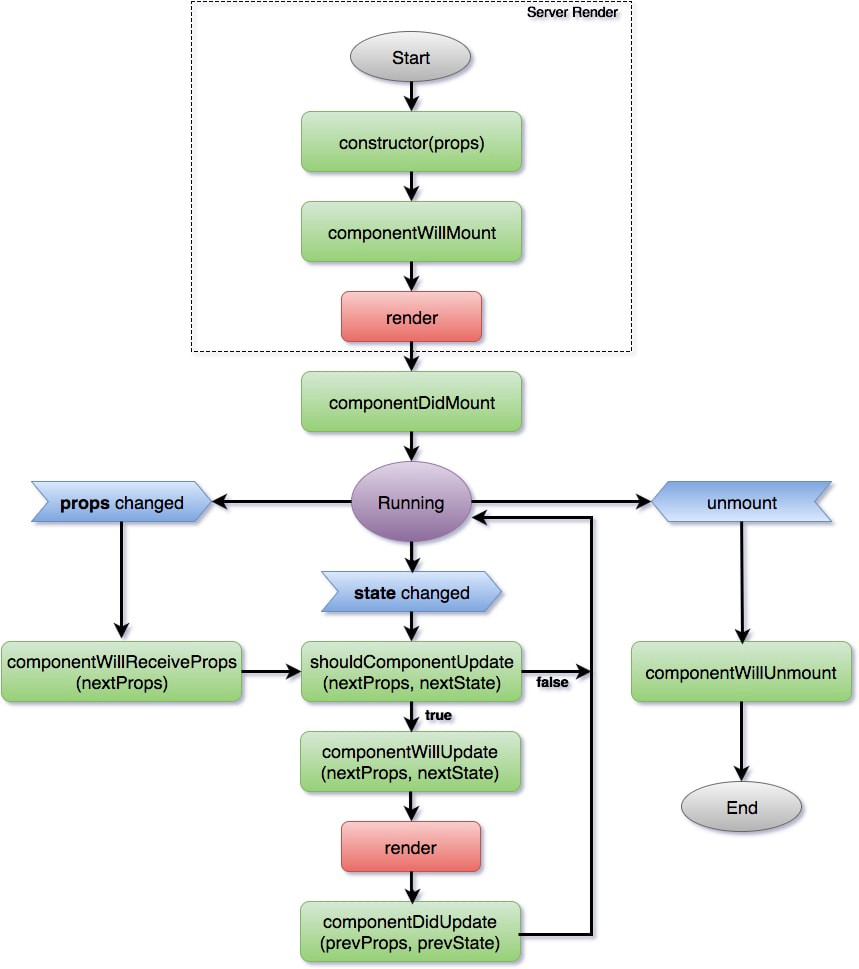
\includegraphics[height=0.60\textheight, keepaspectratio]{img/client/Lifecycle.jpeg}
	\captionsetup{justification=centering, format=plain}
	\caption[Der Lebenszyklus von React]{Der Lebenszyklus von React \\ \quelle \cite{reactLifeCycle}}
	\label{fig:ReactLifecylce}
\end{figure}
